\documentclass[12pt]{article}%
\usepackage{amsfonts}
\usepackage{fancyhdr}
\usepackage{comment}
\usepackage[a4paper, top=1cm, bottom=1.5cm, left=2cm, right=2cm]%
{geometry}
\usepackage{graphicx}% demo option just for the example
\usepackage{caption}
\usepackage{enumitem}
\usepackage{times}
\usepackage{changepage}
\usepackage{amssymb}

\begin{document}

\title{Rotation Project Notes}
\author{Cole \& David}
\maketitle

\subsection{8 May 2025}
\textbf{Next Steps}
\begin{itemize}
    \item To check that convergence actually works, we can do a check by: drawing patch weights (with 10,000 patches) and sum them all up, then check the average deviation from the expected value (which is 1), and we would want to see that the average deviation goes to zero as the patch weight goes up. 
    \begin{itemize}
        \item so the $(actual sum - 1)^2$ gives you the gross deviation, which will probably grow with n, but the average deviation per-patch should shrink with growing n 
        \item can also take $|(actual sum - 1))|$, but they might converge at different rates
        \item try a couple values of q 
        \item plot this on a log(n) scale
    \end{itemize}
    \item to show the shape of how long until I=0, we can run across a geometric number of R0 values (i.e. 0.1 - 10) and this will show an S-shape
    \begin{itemize}
        \item we do want to do this so we can compare between the different things -- constant weights vs. variable weights. 
        \item we want to plot these two things -- the calculated R0 values that we see
        \item re-expressing the R0 we get from patch variability is a sufficient way to characterize an epidemic - if there's still a lot of variance there, then the R0 is not capturing all the variance there 
        \item 
    \end{itemize}
\end{itemize}

\textbf{Next Steps}
\begin{itemize}
    \item look at the different r0s and see how that changes the results
    \item pick a basic r0 and expand around the basic uniform distribution -- does it look like just shifting the r0 by like changing the number of susceptibles 
    \item if they look the same, then if you can understand r0 thats' the key 
    \item if r0 goes up, once you have the bimodality, how many ones go to zero immediately, track that? 
    \item if r0 goes up because you're changing the patch heterogeneity
\end{itemize}

\subsection{24 April 2025}

\textbf{Next Steps}
\begin{itemize}
    \item look at the different r0s and see how that changes the results
    \item pick a basic r0 and expand around the basic uniform distribution -- does it look like just shifting the r0 by like changing the number of susceptibles 
    \item if they look the same, then if you can understand r0 thats' the key 
    \item if r0 goes up, once you have the bimodality, how many ones go to zero immediately, track that? 
    \item if r0 goes up because you're changing the patch heterogeneity
\end{itemize}

\subsection{27 February 2025}

\textbf{Notes:}
\begin{itemize}
    \item  we could bring in Zach to help us with some of the math stuff 
    \begin{itemize}
        \item would give us a clearer interpretation of what kind of metric we would actually want 
        \item in step 1 of the introduction of the disease we get a probability of it going to step 2, but we want to be able to say with some certainty that the epidemic will "succeed" -- would be nice to find a way to integrate across a number of timesteps -- we could design a threshold to say like "under this scenario, the progression of an epidemic will happen with some probability"
        \item would be harder in the analytical side to do some sort of "death" term 
    \end{itemize}
    \item we could do something simulation-based on the other side and gives you some weird tail of patches that are "habitable" 
    \item if we can look at a given start point and find the probability that it does go to an epidemic
    \item we want to do something analytically that approaches $R_0$
    \item think about whether or not there are simpler distributions that we could use that would give us a simpler outcome -- maybe a log-normal? maybe gamma? the uniform is clear which is nice so maybe we stick with that 
    \begin{figure}[!hpt]
        \centering
        % \includegraphics[width=0.65\linewidth]{notes-figs/XXXXXX.jpg}
        \caption{}
    \end{figure}
\end{itemize}

\textbf{Next Steps:}
\begin{enumerate}
    \item in the numerical side of things: 
    \begin{itemize}
        \item develop a simple set of code to run through what we've just decided on, tinker with the code and see what goes ! 
        \item re-write some of the overleaf so that it's something we can show to zach and ask for help with 
        \item David will try for $I=2$
        \item i will also try and work through the solutions long-hand / with steps explicit to see what it shows 
    \end{itemize}
\end{enumerate}

\subsection{30 January 2025}
\textbf{Notes:}
\begin{itemize}
    \item code up a set of 100 patches with $w_ij= 1/100$ and just see what we get 
    \item random placement of individuals and see how frequently you get co-location, and then see which of the equations are right -- many many simulations
    \item then you can do it with some heterogeneous options 
    \item they should converge -- just need to do it many many times over 
    \item choose a random value out of the list given the weights and that's where your S lands, and then do it again for as many S's as you have, then do it again for the I -- see is what you chose randomly for your I individual is the same as where the S's are -- if it does then that's a "yes" and we can do this 1 million times 
\end{itemize}
\textbf{Next Steps:}
\begin{enumerate}
    \item Cole will code up a set of simulations to see if our derivation is correct, by using a set of w values that are the same (100 cells), and checking if the predicted values from our derivation 
    \item then Cole will repeat this with some heterogeneous options. using this pseudocode 
\end{enumerate}
\begin{figure}[!hpt]
    \centering
    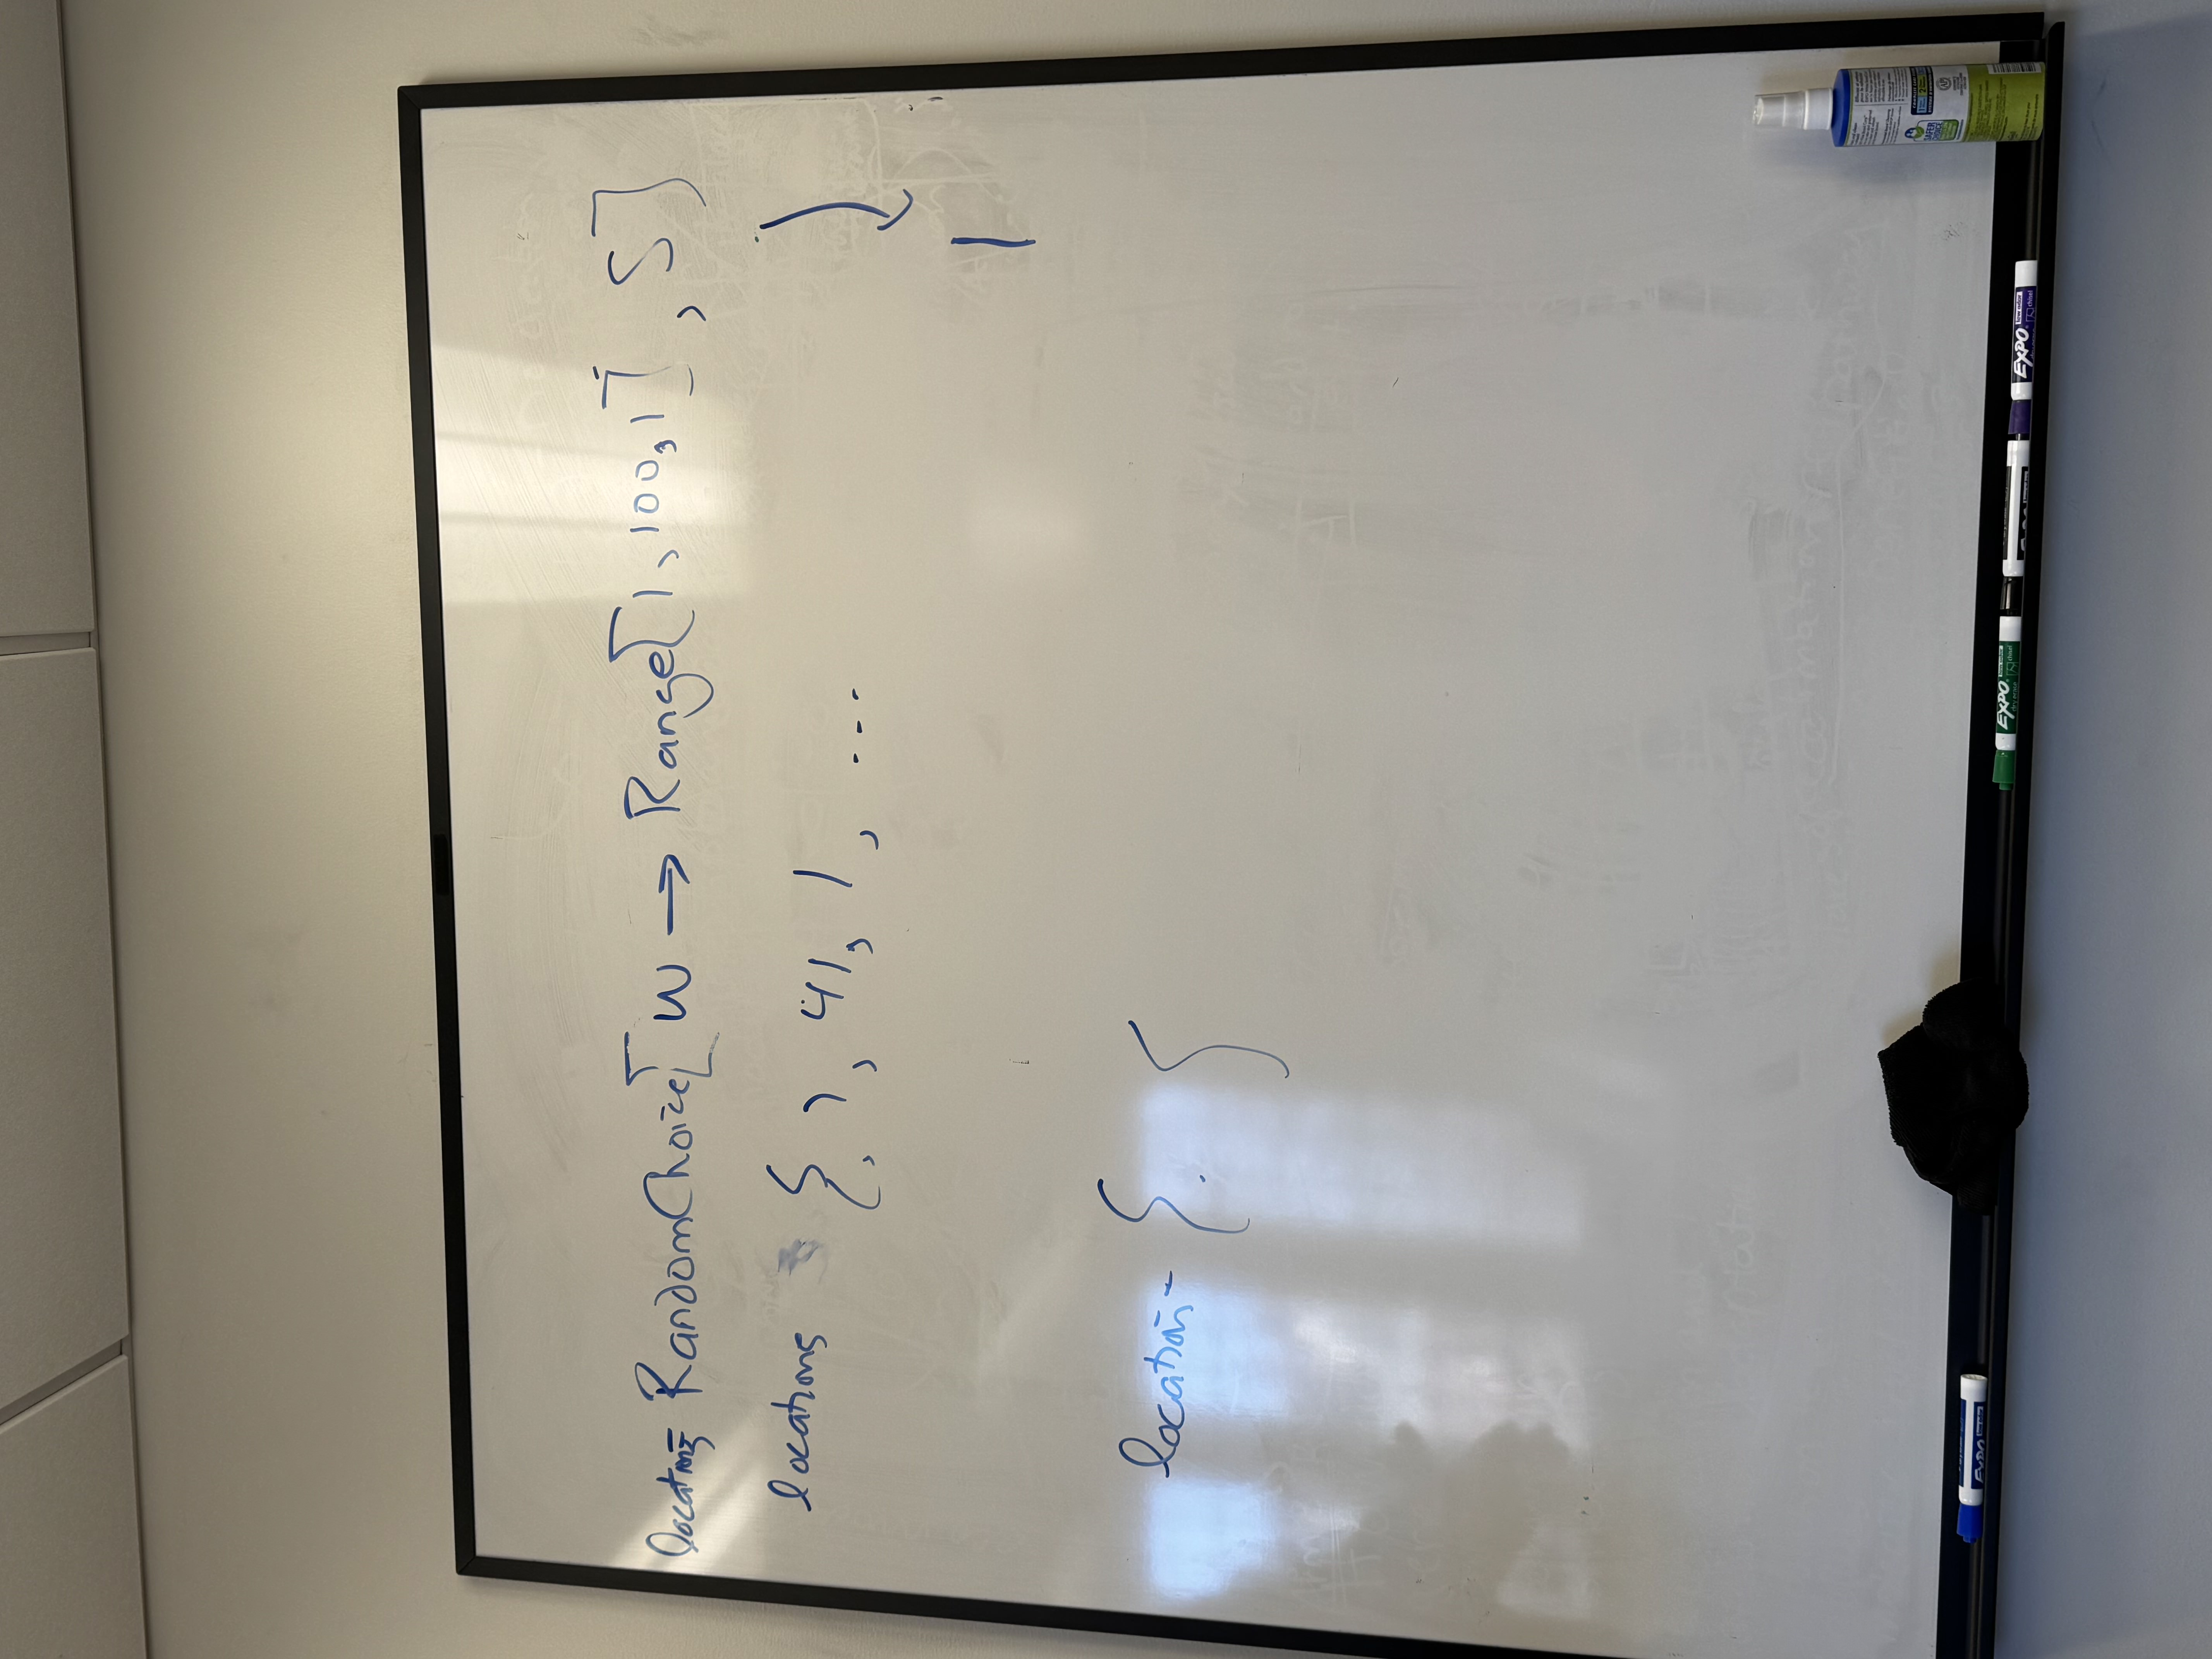
\includegraphics[width=0.65\linewidth]{notes-figs/20250130-pseudocode.jpg}
    \caption{Psuedocode of how to do the simulation to check equivalency stuff, particularly the choice of the where the random values go for S and I -- the random placement}
\end{figure}


\subsection{12 December 2024}

\textbf{Notes:}
\begin{itemize}
    \item we want to move towards thinking of our limits as "endpoints" of heterogeneity 
    \begin{itemize}
        \item everything is homogenous is one end point (all of the probabilities are equal), so the sum that you take is just all $w_{ij}$ with the same values 
        \item if everything is maximal heterogeneity -- no matter how many patches on the landscape there are, there's only one patch that organisms find their way to 
        \item highest contact rates are in the maximum heterogeneity, lowest in the maximal homogeneity
    \end{itemize}
    \item in terms of coupling the supply and temperature, they need to be independent distributions with a covariance term -- so given the model, you have $\mathbf{\phi}$ and then the variance of each of the two parameters $\sigma^2_T$ and $\sigma^2_S$ -- we have to now think about how changing some variance parameter (T, for example) changes that $\mathbf{\phi}$. We could think of it like: 

\begin{figure}[!hpt]
    \centering
    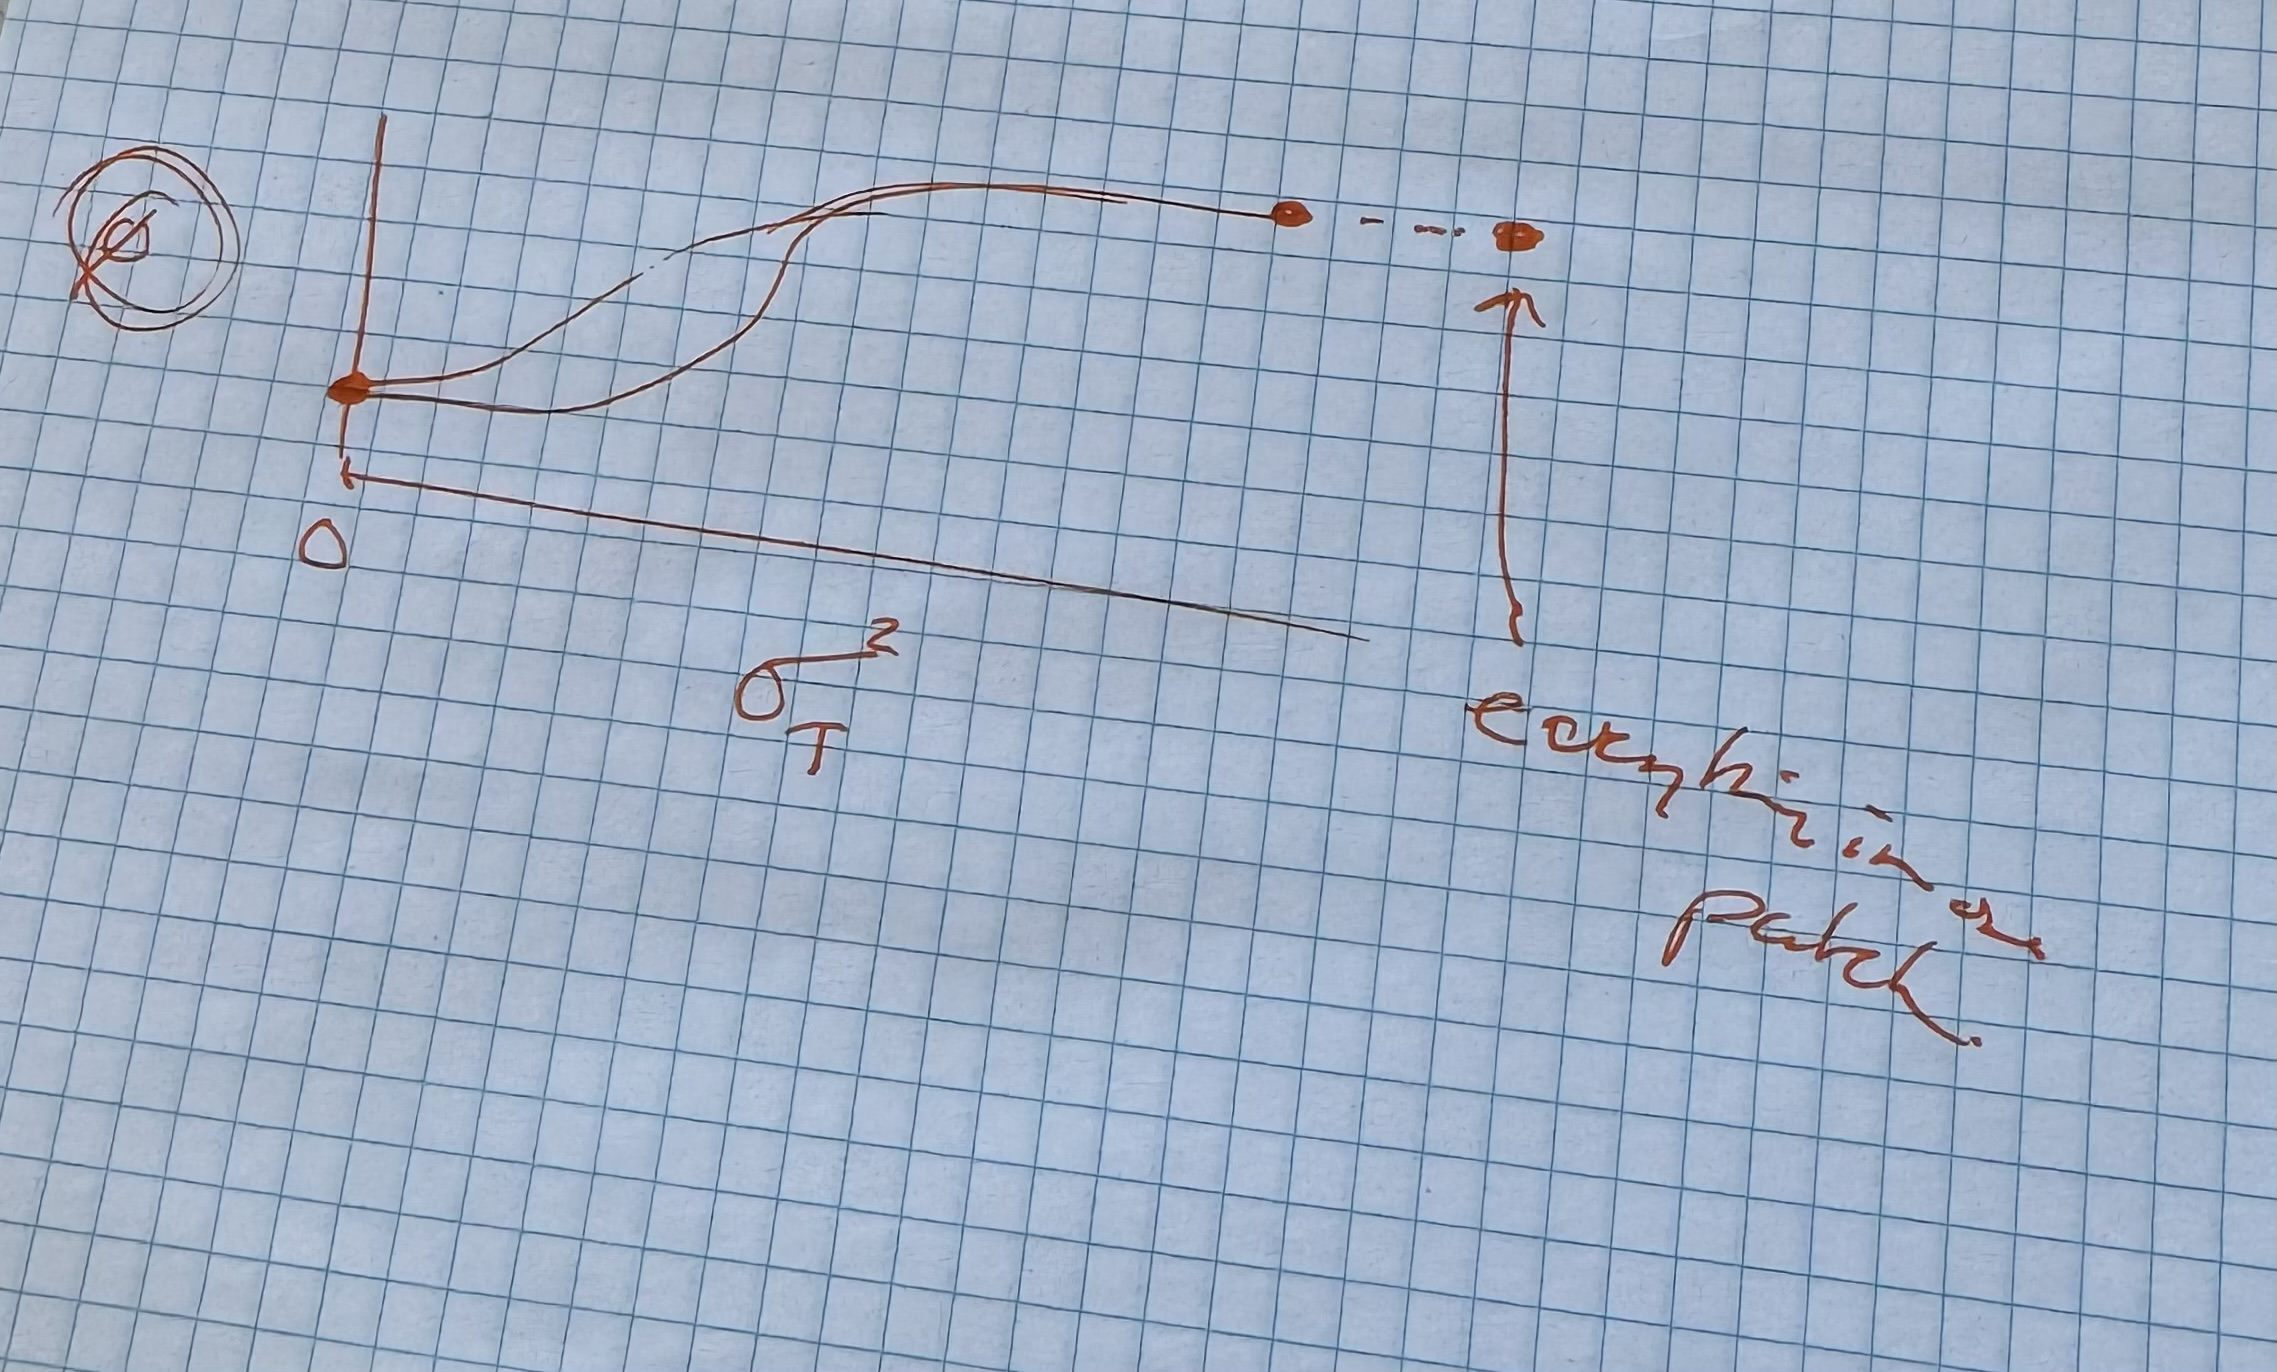
\includegraphics[width=0.65\linewidth]{notes-figs/phi-sigma-t.jpg}
    \caption{expectation of changing the sigma term and the response in $\phi$. Additionally, you can imagine the asymptote shifting if the background changes.}
\end{figure}

\item you can also imagine that there's a plot that shows the grid of the two values and you pick some sort of grid and look at these two parameters independently, and then look at the correlation between the two $\sigma$ values, something like this: 

\begin{figure}[!hpt]
    \centering
    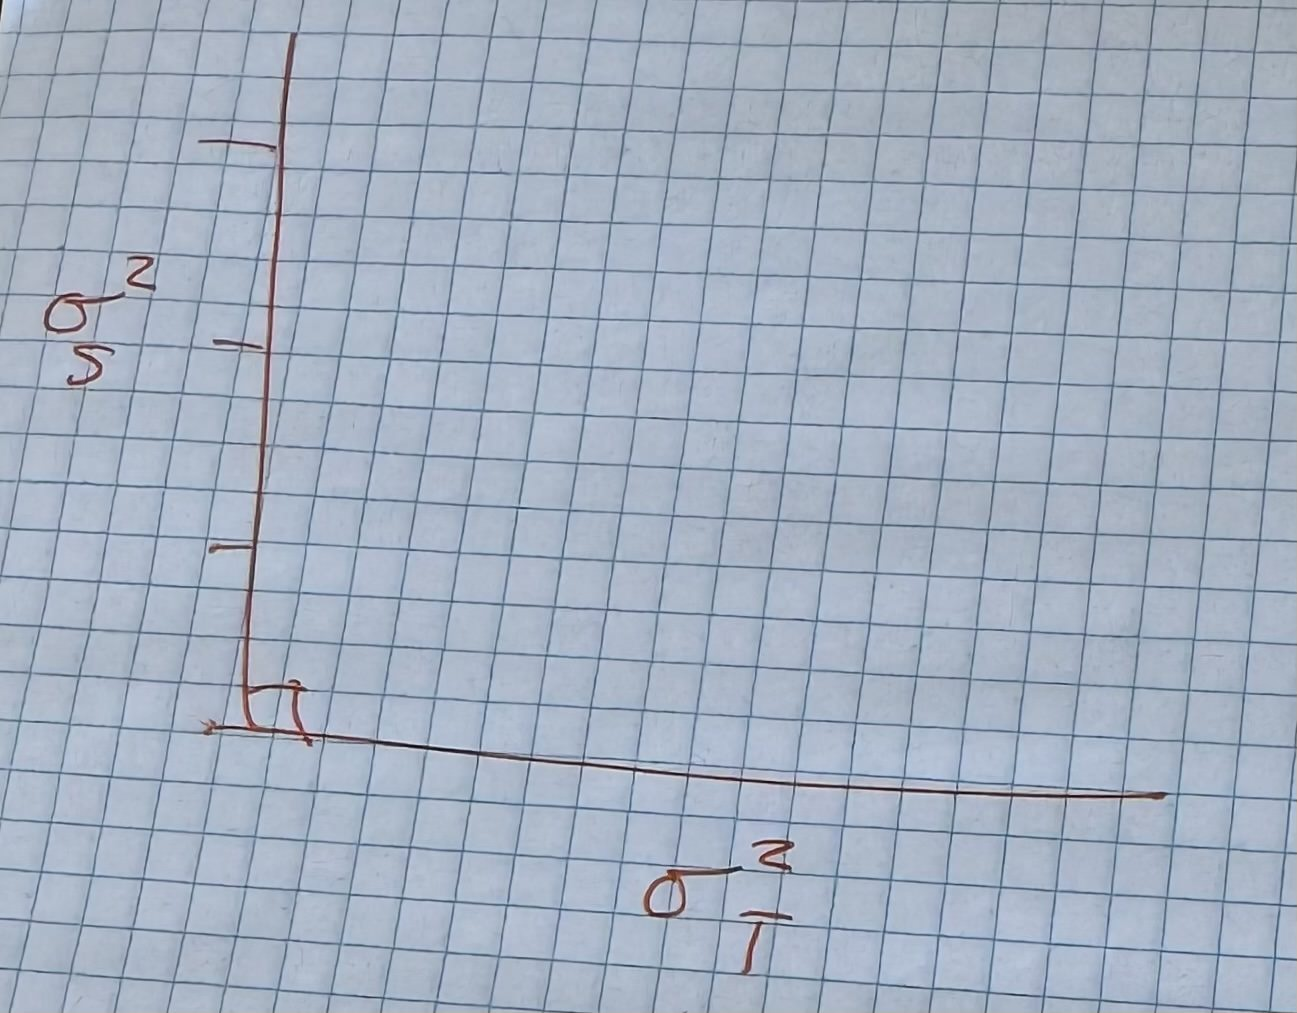
\includegraphics[width=0.65\linewidth]{notes-figs/sigma-vs-sigma.jpg}
    \caption{Some grid of $\sigma$ values that relate one to the other that shows how spatial heterogeneity relates to temperature heterogeneity and what that means for our response. This is going to be filled with $\mathbf{\phi}$}
\end{figure}

\item could change the S value, change the number of Susceptible individuals, the number of infecteds, and the qualitative shape of the sigmoidal curve above should just shift down, it shouldn't change qualitative 
\item we want to take the measure of $\phi$ a bit deeper, ideally moving towards like the idea of doing expectations and expected values or take it through a few of the steps to be able to say "what is the probability of moving from one infected to 10 infected individuals" or something of that nature. 
\item we want to take this to the point where we can simulate it outwards, and hone in the notion of spatial heterogeneity and how that generates a "super spreader" effect 
    \begin{itemize}
        \item we would want to be able to think a bit deeper about how this thermal / spatial heterogeneity is changing -- how can this interact to global change? 
        \item we could try and say something about how this would be helpful for pulling apart the effects of thermal / spatial heterogeneity because they likely have different effects in different directions 
    \end{itemize}
\end{itemize}

\textbf{Next Steps:}
\begin{enumerate}
    \item Explore the parameter space for the above notes related to the sigmas 
    \item there's a possibility of moving this beyond just a theoretical lens (see voice note from Dec 12, 2024, around 16mins to see David's thoughts on this) 
\end{enumerate}

\end{document}